\documentclass{article}

% if you need to pass options to natbib, use, e.g.:
% \PassOptionsToPackage{numbers, compress}{natbib}
% before loading nips_2016
%
% to avoid loading the natbib package, add option nonatbib:
% \usepackage[nonatbib]{nips_2016}

% % \usepackage{nips_2016}

\PassOptionsToPackage{numbers, compress}{natbib}

% to compile a camera-ready version, add the [final] option, e.g.:
\usepackage[final]{nips_2016}

\usepackage[utf8]{inputenc} % allow utf-8 input
\usepackage[T1]{fontenc}    % use 8-bit T1 fonts
\usepackage{hyperref}       % hyperlinks
\usepackage{url}            % simple URL typesetting
\usepackage{booktabs}       % professional-quality tables
\usepackage{amsfonts}       % blackboard math symbols
\usepackage{nicefrac}       % compact symbols for 1/2, etc.
\usepackage{microtype}      % microtypography
\usepackage{natbib}
\bibliographystyle{unsrtnat}
\usepackage{graphicx}
\usepackage{amsmath}

\title{An oscillatory neural network model of motor dynamics during continuous periodic movement}

% The \author macro works with any number of authors. There are two
% commands used to separate the names and addresses of multiple
% authors: \And and \AND.
%
% Using \And between authors leaves it to LaTeX to determine where to
% break the lines. Using \AND forces a line break at that point. So,
% if LaTeX puts 3 of 4 authors names on the first line, and the last
% on the second line, try using \AND instead of \And before the third
% author name.

\author{
  Iran Roman\\
  Stanford Neuroscience Graduate Program\\
  Center for Computer Research in Music and Acoustics\\
  Stanford University\\
  Stanford, CA 94305 \\
  \texttt{iran@stanford.edu} \\
  %% examples of more authors
\And
Wisam Reid \\
  Center for Computer Research in Music and Acoustics\\
  Stanford University\\
  Stanford, CA 94305 \\
  \texttt{wisam@ccrma.stanford.edu} \\
  %% Affiliation \\
  %% Address \\
  %% \texttt{email} \\
  %% \AND
  %% Coauthor \\
  %% Affiliation \\
  %% Address \\
  %% \texttt{email} \\
  %% \And
  %% Coauthor \\
  %% Affiliation \\
  %% Address \\
  %% \texttt{email} \\
  %% \And
  %% Coauthor \\
  %% Affiliation \\
  %% Address \\
  %% \texttt{email} \\
}

\begin{document}
% \nipsfinalcopy is no longer used

\maketitle

\begin{abstract}
Brain oscillations are of functional relevance to the healthy functioning of the brain. In the motor system, desynchronization of oscillatory activity in the beta band (~20Hz) is observed through periodic somatosensory and/or auditory stimulation. This desynchronization occurs at a rate equal to the period of stimulation, and resynchronization of oscillatory activity anticipates the next stimulus. The computations underlying motor function can be explained by networks of neural oscillators carrying out non-linear transformations of stimuli, reflected by desynchronization of oscillatory activity in the motor system. We developed a neural model of nonlinear oscillators that transforms stimuli into characteristic oscillatory activity of the beta band. Our model is built using a canonical model of nonlinear oscillators, captures even-related desynchronization in the beta band, and is able to anticipate the next period of stimulation through resynchronization. Additionally, our model provides a dynamical-systems perspective of computations and stimuli transformations in the motor system.
\end{abstract}

\section{Introduction}

The brain exhibits patterns of rhythmic activity known as brain oscillations. Such oscillations exist around characteristic frequency bands (2-3Hz, 5Hz, 10Hz, 20Hz, 40Hz, 80Hz), and have been observed in humans as well as in other animals \cite{giraud2012cortical}. 

\subsection{Functionality of brain oscillations}

Research has shown that brain oscillations have functional roles in cognition and signal processing throughout the brain \cite{sejnowski2006network}. For example, these oscillations modulate the rate at which small populations of neurons fire \cite{engel2001dynamic}, and they can also dynamically coordinate processes throughout the brain \cite{varela2001brainweb} \cite{engel2010beta}. The beta band, which comprises the rates of oscillation centered around 20Hz (between 13Hz and 30Hz) \cite{engel2010beta}, is important for function and coordination throughout the motor system. For example, when a human taps periodically the beta band loses energy shortly after every tap due to an event related desynchronization (ERD). After the ERD, the oscillators in the beta band resynchronize to reach their original amplitude at the moment when the next tap arrives \cite{fujioka2012internalized}. This is an example of a higher-order brain process (here anticipation of the next stimulus) that is reflected by brain oscillations (see Figure \ref{fig:ERD}). However, one could question whether brain oscillations are just the "exhaust fumes" of lower-level processes throughout the brain. Evidence has shown that, the beta band in the motor system is of major functional significance. Patients suffering from Parkinson's disease do not show normal ERDs \cite{magnani1998event}. However, deep brain stimulation with frequencies corresponding to the gamma band (80Hz) improves motor function in Parkinson's patients. This demonstrates the causal relationship between brain oscillations and normal brain functioning \cite{swann2011deep}.

\begin{figure}
  \centering
  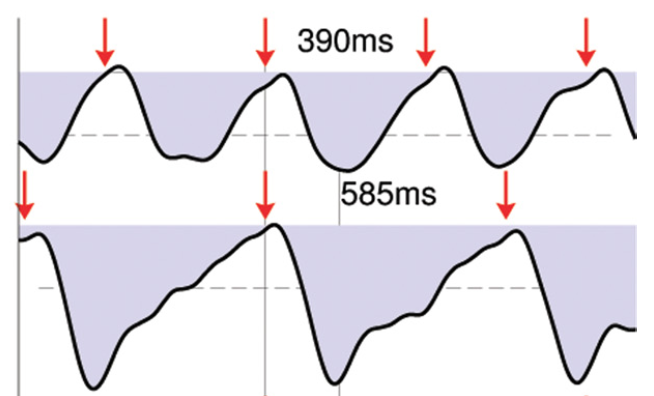
\includegraphics[scale=0.75]{betaERD.png}
  \caption{ERD of oscillatory activity in the beta band during periodic  stimulation at two different periods (390ms and 585ms). Red arrows indicate pulses of stimulation. Notice how the rising slope of the resynchronizing beta band reaches its original peak at the moment when the next stimulus is expected. Modified from \cite{fujioka2012internalized}}
  \label{fig:ERD}
\end{figure}

\subsection{Mechanisms of brain oscillations}

Recent research efforts have tried to elucidate how brain oscillations emerge and propagate across areas in the brain. In primary sensory areas, nonlinear transformations of the input have explained the physiology and processing at the cochlea, and the inferior colliculus \cite{lerud2014pitch}. Current theoretical views about the brain explain neural mechanisms as dynamical systems \cite{izhikevich2007dynamical}. Research along these theoretical lines will likely continue explaining the underlying computations that give rise to oscillations and their functions throughout the brain.

\section{Related work}

Modeling of the motor system has a long history starting with the use of simple model organisms to study motor processes and function throughout the body \cite{rizzolatti2001cortical}. More recently, the momentum around neural networks has led to the development of architectures that capture the dynamics and function of neural processes in the motor system at different levels. A recent model of the motor system has explained the healthy and Parkinsonian states using spiking neural networks and neural fields \cite{kerr2013cortical}. Although highly informative about the interactions between oscillations and neuron spikes, this model was relatively complicated and computationally expensive. Another recent neural network model of the motor system uses a canonical model of nonlinear oscillators in a gradient of frequencies. This model is able to explain the non-linear transformations that stimuli undergo from the auditory to the motor cortex \cite{large2015neural}. Two major features of this neural network are: 1) its ability to abstract information about periodic stimulation, even when such information was missing in the stimulus, and 2) its computational unit, which was a canonical model of a nonlinear oscillator sitting at a Hopf bifurcation \cite{large2010canonical}. Since the model contains units at a Hopf bifurcation in a gradient of frequencies, the input makes certain oscillators resonate and potentially leap across qualitatively different dynamical states. At different dynamical states, the network of canonical oscillators is able to explain memory, learning, and nonlinear transformations that stimuli undergo across layers of computation \cite{large2010canonical}. Thus, we propose that a network of canonical nonlinear oscillators will be able to capture the patterns of ERD and ERS (event related synchronization) in the beta band associated with healthy motor function.

\section{Data processing}

7 Subjects listened a periodic beat at three different speeds while sitting comfortably in a chair and their brainwaves were recorded with a Magnetoencephalogram (MEG). The raw data was epoched to the onset of each beat, and an average response was generated by averaging the response across all beats that they listened. This average is known as the event related potential (ERP). A wavelet transform was applied to the ERP in order to obtain the oscillatory brain responses phase-locked to the onset of the stimulus. The resulting response is known as the evoked response. Additionally, the induced response was obtained by applying the wavelet transform to individual trials of beat listening, and subtracting the evoked response from each one of the individual trials. The beta band of activity was selected by band-pass filtering and averaging the time-series for oscillatory activity between 18 and 23 Hz. A z-score was applied to the beta band resulting in a series of data depicting power fluctuations over time, similar to Figure \ref{fig:ERD}.

\begin{figure}[t]
  \centering
  \hspace*{-0.75cm}   
  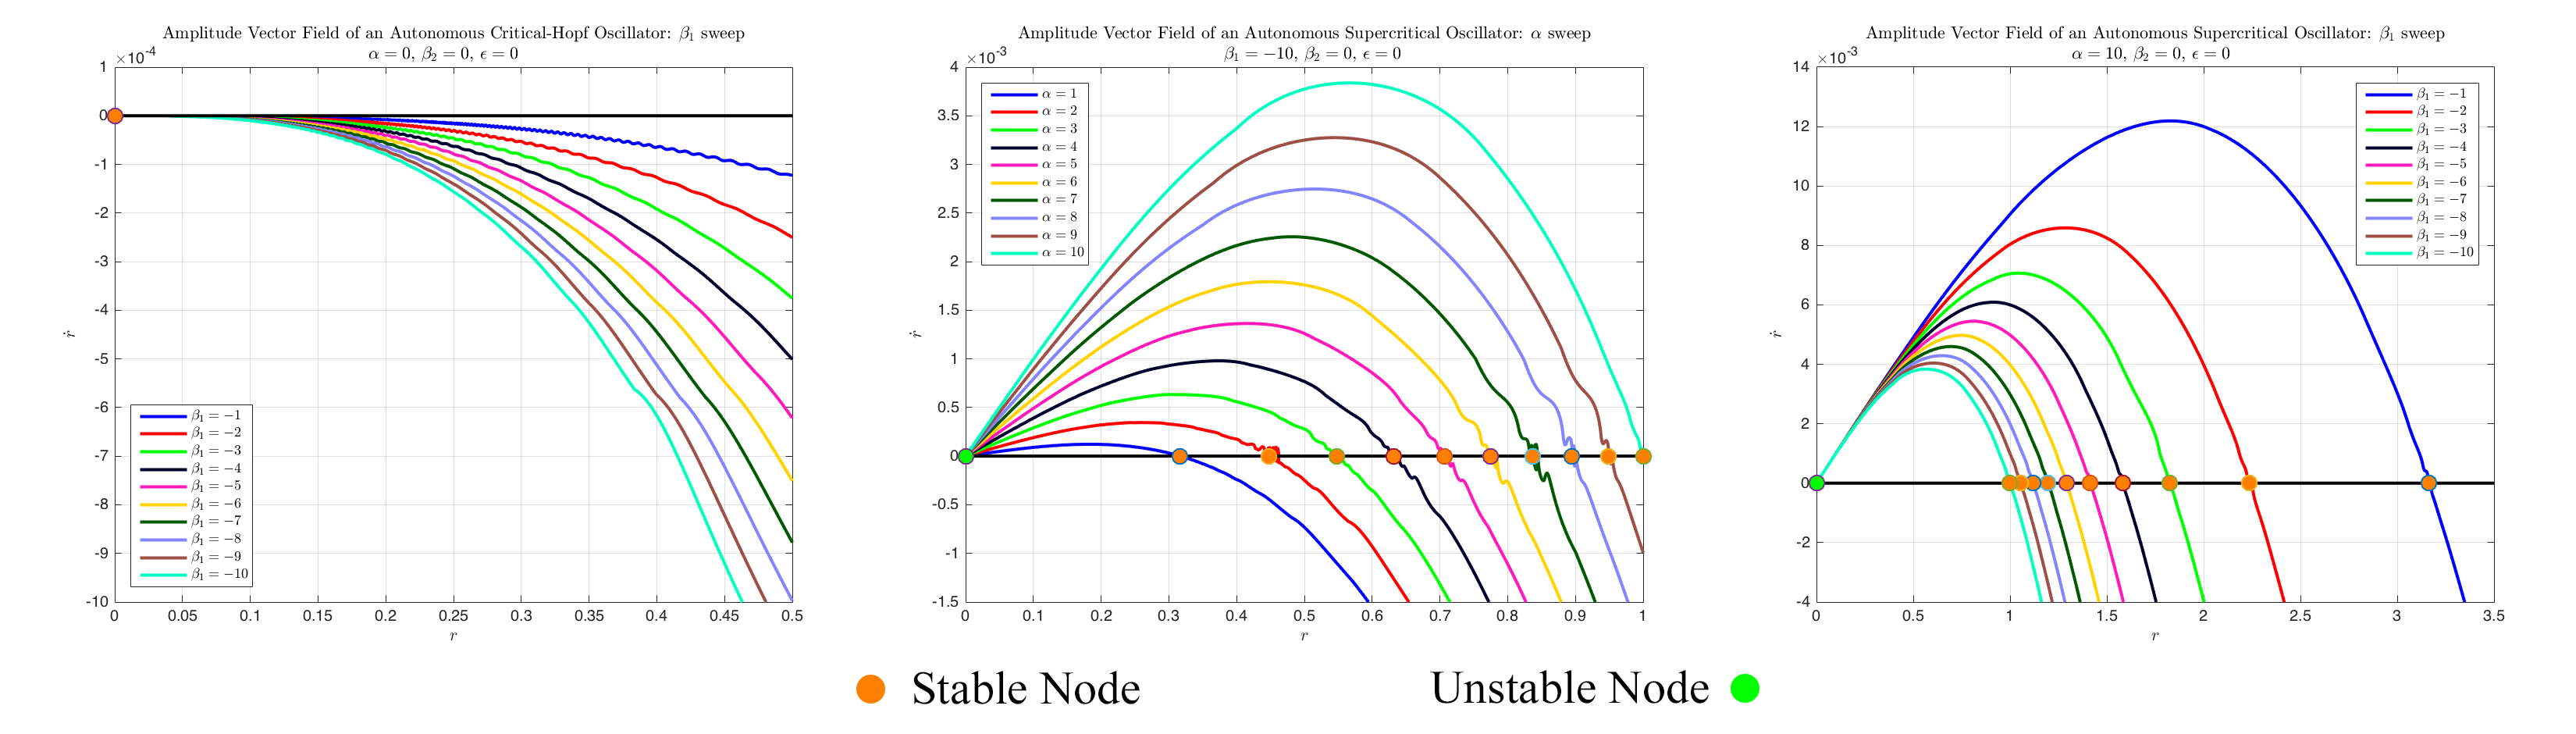
\includegraphics[scale=0.13]{sub_super_Critical.png}
  \caption{Amplitude vector field (AVF) for the critical Hopf regime (Hopf bifurcation) sweeping through several values of $\beta_1$ (left). AVF for the supercritical Hopf (limit cycle) regime sweeping through several values of $\alpha$ (center) and $\beta_1$ (right). Orange circles indicate stable fixed points (attractors) and green circles unstable fixed points (repellers).}
  \label{fig:sub_super}
\end{figure}

\section{Methodology}
% TODO by WISAM
% don't forget: mention that stimulation of all our models was a real-valued impulse
We built a model using canonical nonlinear neural oscillators described by the ordinary differential equation: 
\begin{equation}
\dot{z} = z\bigg( \alpha + i\omega +\beta_1|z_i|^2+\frac{\epsilon\beta_2|z_i|^4}{1-\epsilon|z_i|^2}\bigg)
\end{equation}

% \begin{wrapfigure}{R}{0.5\textwidth}
% \centering
% 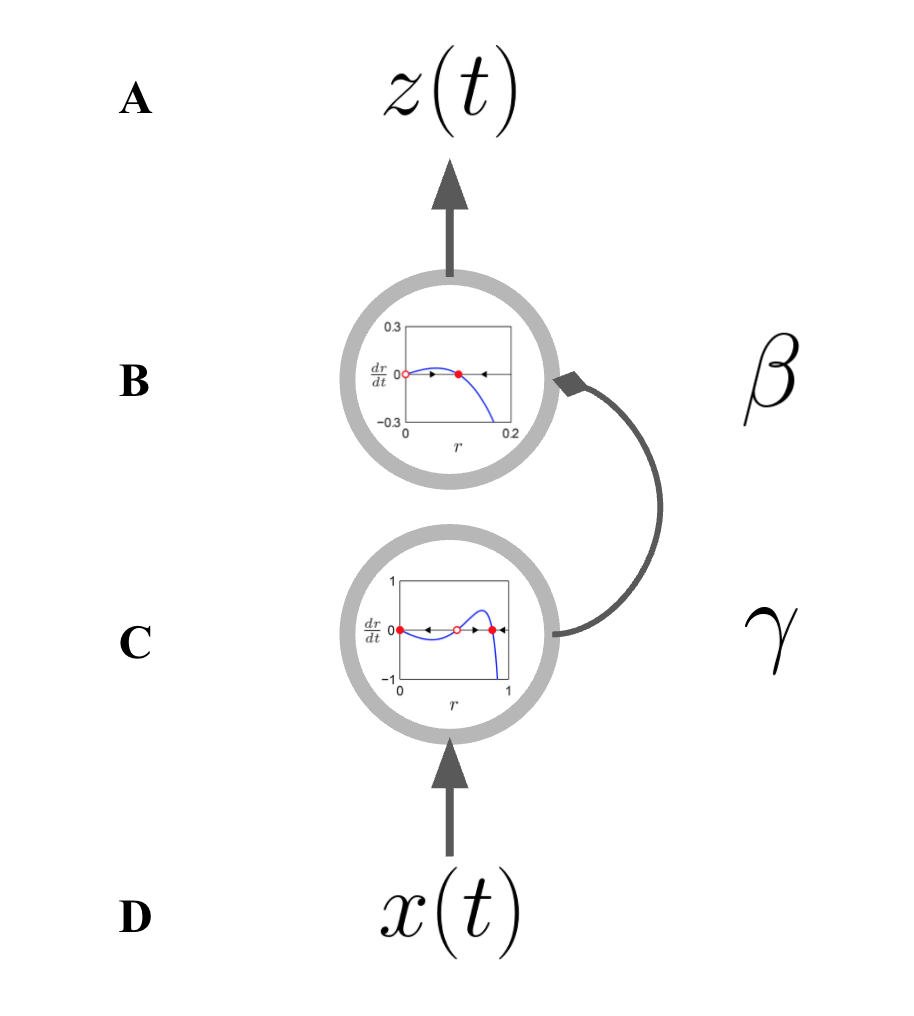
\includegraphics[width=0.4\textwidth,right]{model1.png}
% \caption{\label{fig:arch}System dynamics with isochronous stimulation}
% \end{wrapfigure}

where $z(t)$ is a complex state variable containing amplitude and phase information ($z = re^{i\phi}$), $\omega$ is the natural frequency of oscillation, and the parameters that determine the dynamical properties of the oscillator are $\alpha$, $\beta_1$, $\beta_2$, and $\epsilon$ controlling the bifurcation of autonomous behavior \cite{large2010canonical}\cite{kim2015signal}.  The high-order terms govern the non-linear properties of an oscillator, which can be driven by an external input or by other oscillators in the network. 

A great advantage of the canonical model, beyond its ability to capture generic properties of oscillation, is it's simple mathematical form amendable to fixed-point analysis (i.e. analysis of its steady state dynamics). However, it is still difficult to analyze the network in its entirety because its dynamics are determined by complex interactions among multiple network components.  Our approach began with a dynamical systems analysis of the autonomous behavior of our canonical model, examining individual components of the network separately. Using fixed-point analysis we are able to identify various behaviors of canonical oscillators across several ranges of model parameters. The analysis shows that canonical oscillators exhibit qualitatively different sets of states and transitions for different regimes of model parameters. Consistent with previous literature, we were able to distinguish four main categories of parameter regimes, based on their distinct signal processing capabilities \ref{table:regimes}.
% We hope this analysis will aid our understanding of the global network dynamics as a combination of its component dynamics and inform the future automation of oscillatory neural network (ONN) model parameters of auditory signal processing.

\subsection{Autonomous oscillator analysis}
By converting to polar form, the autonomous dynamics of the oscillator (when $F = 0$) can be broken into amplitude and phase components:

\begin{align}
\dot{r} &= \alpha r + \beta_1 r^3 + \frac{\epsilon\beta_2 r^5}{1-\epsilon r^2} \\
\dot{\phi} &= \omega
\end{align}

Here we can see that the phase $\phi$ advances at the constant rate of $\omega$.
Equation (2) defines the amplitude vector field, over which we will do our analysis. We start by solving for the fixed points in the vector field, by solving $\dot{r} = 0$, we then evaluate the stability of each fixed point.  The fixed point stability determines if it is an ``attractor" or a ``repeller", which the oscillator will converge to or diverge from respectively. Depending on the values of $\alpha, \beta_1,$ and $\beta_2$, the autonomous amplitude vector field can have one of four distinct behaviors. These four regimes can be seen in figures \ref{fig:sub_super} \ref{fig:superDLC} \ref{fig:subDLC} and are defined in the table below:

\begin{table}[ht]
  \centering
    \begin{tabular}{ | l | l | }
      \hline
      Bifurcation Regime & Model Parameters  \\
      \hline
      Critical Hopf     & $\qquad \alpha = 0, \beta_1 <0,\beta_2 = 0 \qquad$ \\
       \hline
      Supercritical Hopf     & $\qquad \alpha > 0, \beta_1 < 0,\beta_2 < 0 \qquad$    \\
       \hline
      Supercritical Double Limit Cycle   & $\qquad \alpha < 0, \beta_1 > 0,\beta_2 < 0, ~\text{local max} > 0 \qquad$ \\   
       \hline
      Subcritical Double Limit Cycle     & $\qquad \alpha < 0, \beta_1 > 0,\beta_2 < 0, ~\text{local max} < 0 \qquad$ \\    
      \hline
    \end{tabular}
  \label{table:regimes}
\end{table}

As can be seen in figure \ref{fig:sub_super}, in a critical Hopf regime an oscillator's amplitude decays to zero while oscillating at its natural frequency.  In the supercritical Hopf regime (limit cycle) $\dot{r}$  increases from zero (repelled by the unstable fixed point) and then decreases after a local maximum, toward a stable non-zero fixed point. In the case of a supercritical double limit cycle (DLC) there are three fixed points with two local extrema, two of the fixed points are stable, indicating bistability between equilibrium at zero and spontaneous oscillation at a non-zero amplitude (figure \ref{fig:superDLC}). When the local maximum in the AVF moves below the $r$ axis, by decreasing $\beta_1$, the two non-zero fixed points collide and disappear.

Using the dynamical properties of these oscillators, we built neural networks of non-linear oscillators (ONNs) that will amplify an external input through nonlinear transformations. Such transformed stimulus can be inhibitory input to a limit-cycle oscillator, which after stimulation will resynchronize to its spontaneous amplitude of oscillation. Additionally, delivering a nonlinearly transformed input to a double-limit cycle (DLC) oscillator could make this DLC oscillator transition from a state of spontaneous decay, to a state of spontaneous oscillation. This could lead to a memory state that emerges in our model through periodic stimulation. 

\begin{figure}[t]
  \centering
  \hspace*{-0.75cm}   
  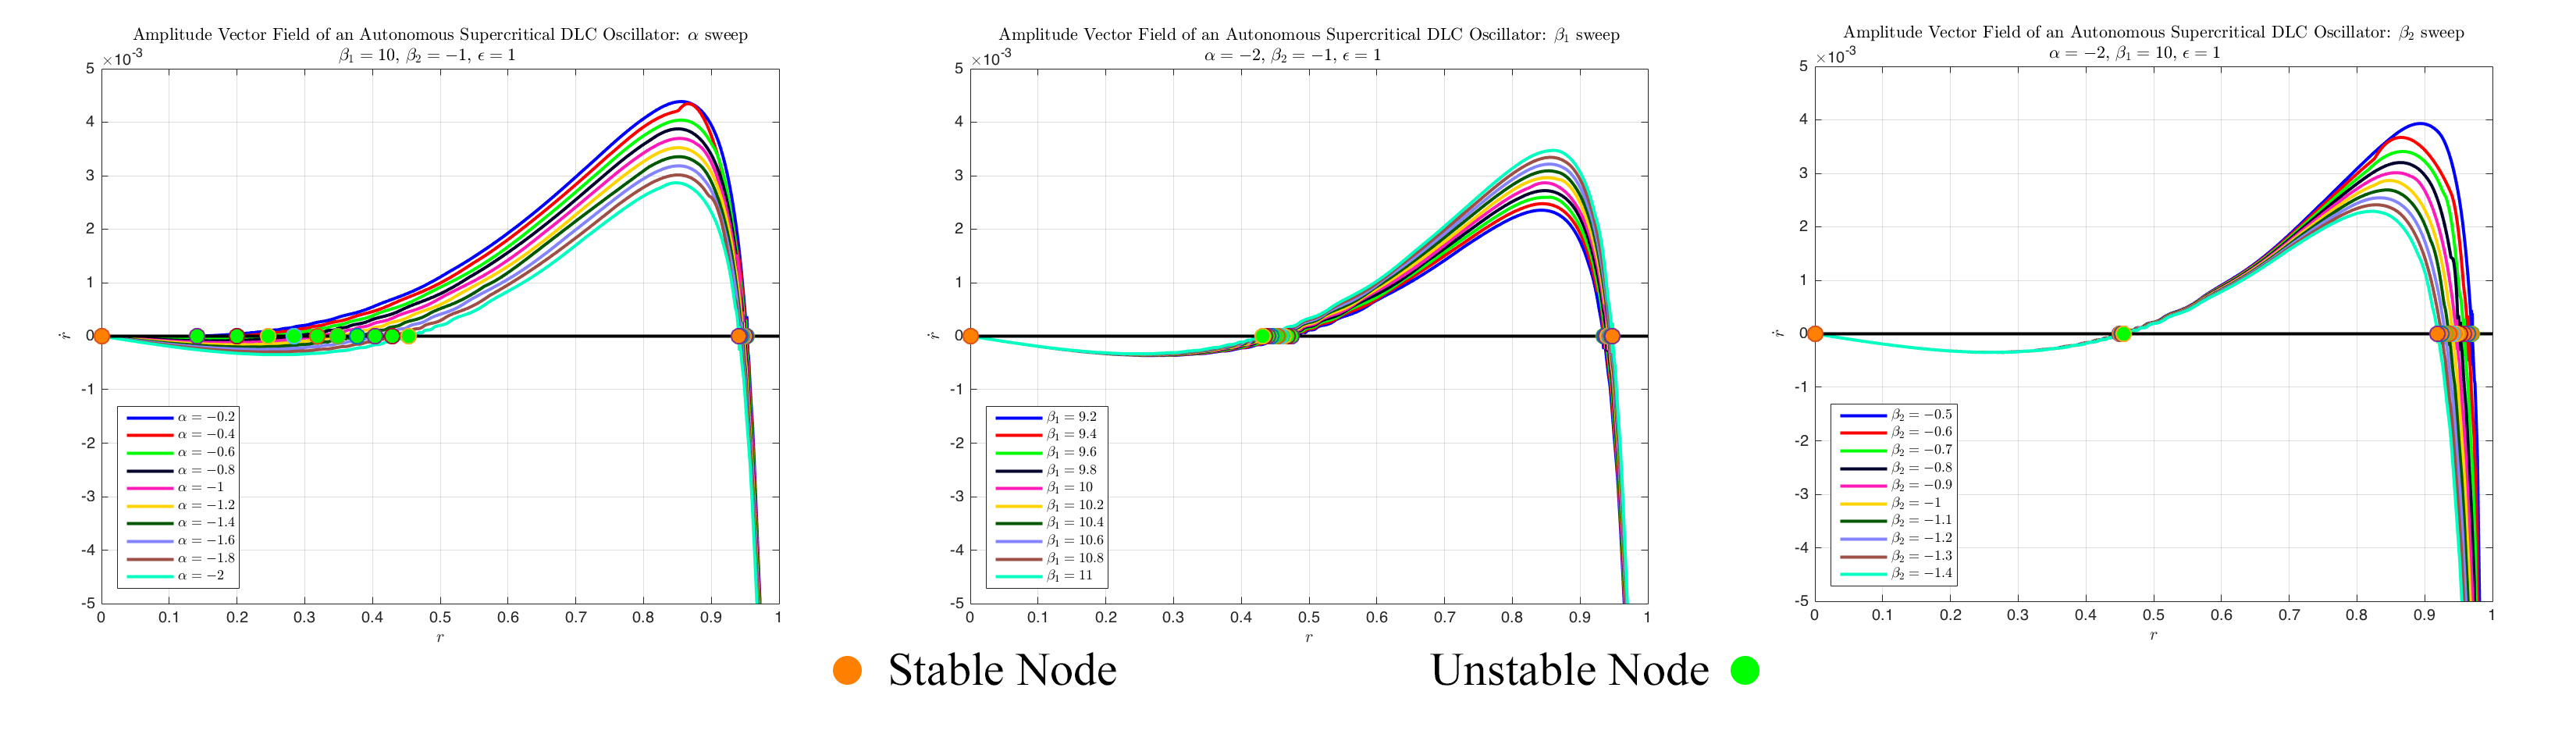
\includegraphics[scale=0.13]{superCritical_DLC.png}
  \caption{Amplitude vector field (AVF) response for the supercritical Hopf DLC regime sweeping through several values of $\alpha$ (left). AVF response for the supercritical Hopf DLC regime sweeping through several values of $\beta_1$ (center). AVF response for the supercritical Hopf DLC regime sweeping through several values of $\beta_2$ (right).} 
  \label{fig:superDLC}
\end{figure}
\begin{figure}[b]
  \centering
  \hspace*{-0.75cm}   
  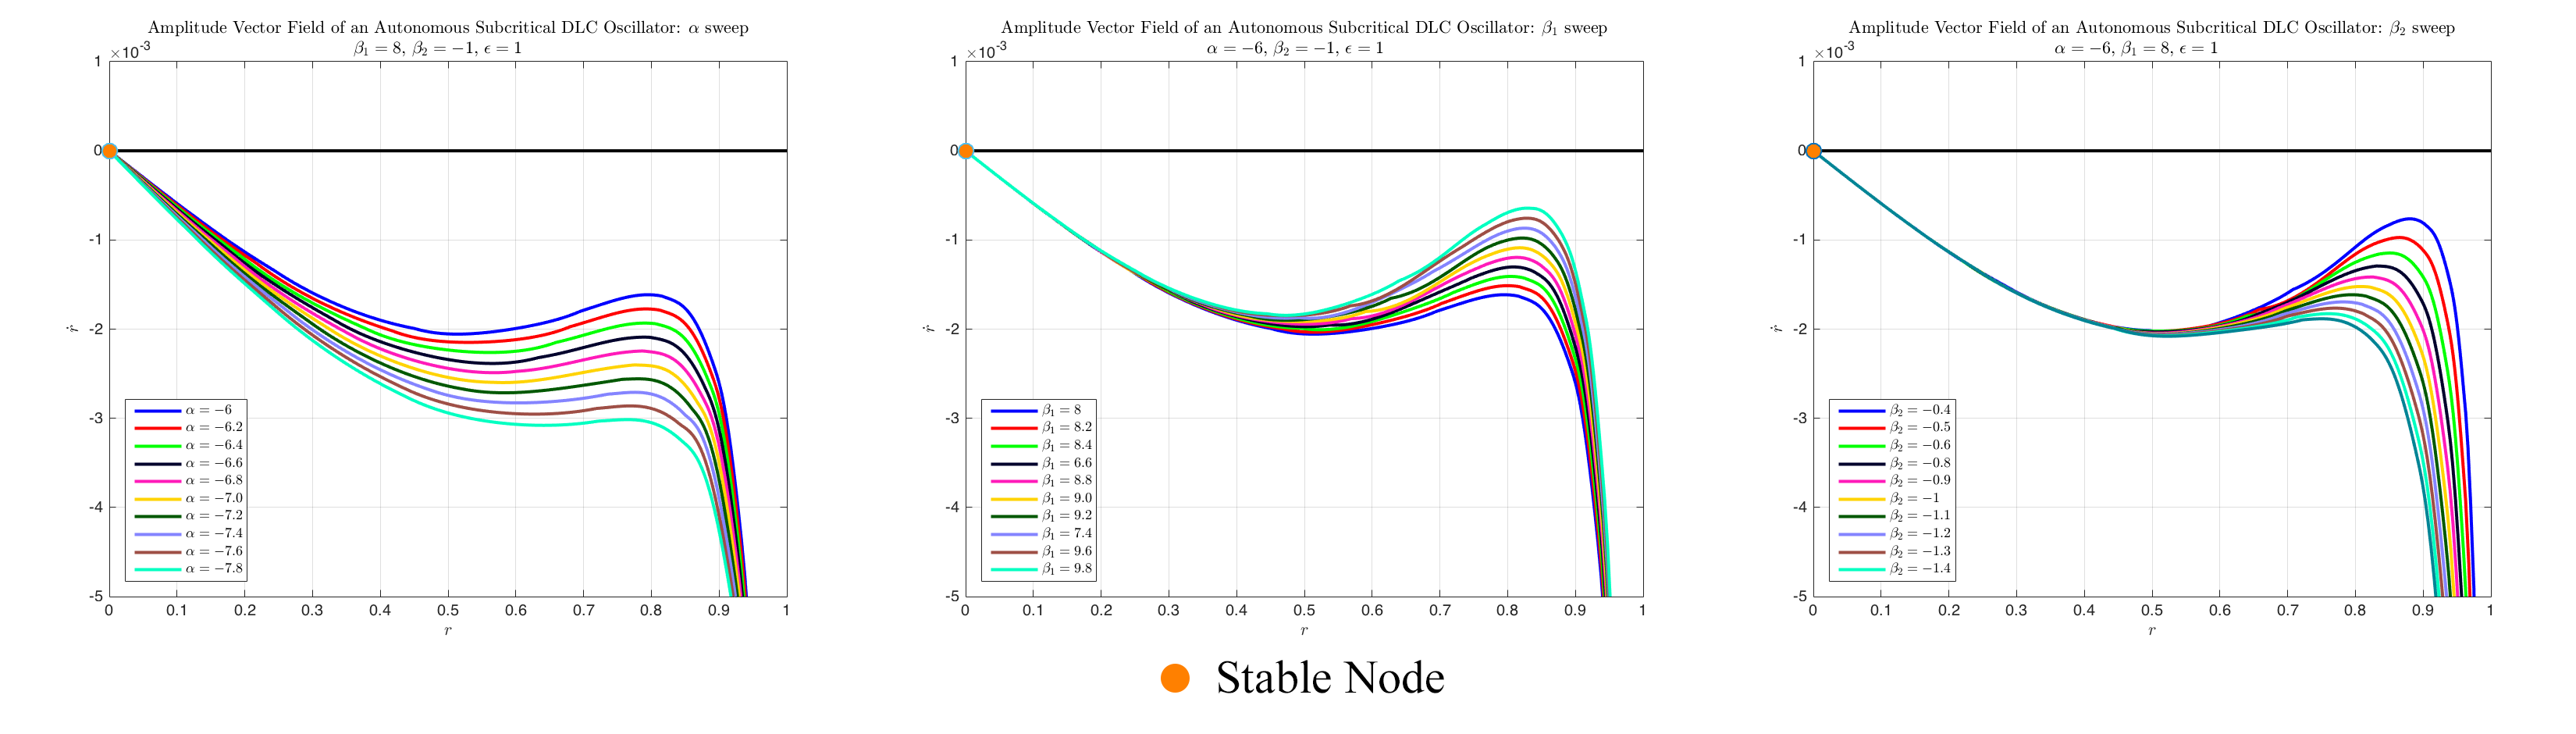
\includegraphics[scale=0.13]{subCritical_DLC.png}
  \caption{Amplitude vector field (AVF) for the subcritical Hopf DLC regime sweeping through several values of $\alpha$ (left).AVF for the subcritical Hopf DLC regime sweeping through several values of $\beta_1$ (center). AVF response for the subcritical Hopf DLC regime sweeping through several values of $\beta_2$ (right).}
  \label{fig:subDLC}
\end{figure}

\section{Architectures and results}

We built and tested a total of three ONN architectures to explain the dynamics of the motor system under periodic forcing. Here is a description of the topology and behavior observed in each one. 

\subsection{Architecture 1}

\begin{figure}[h]
  \centering
  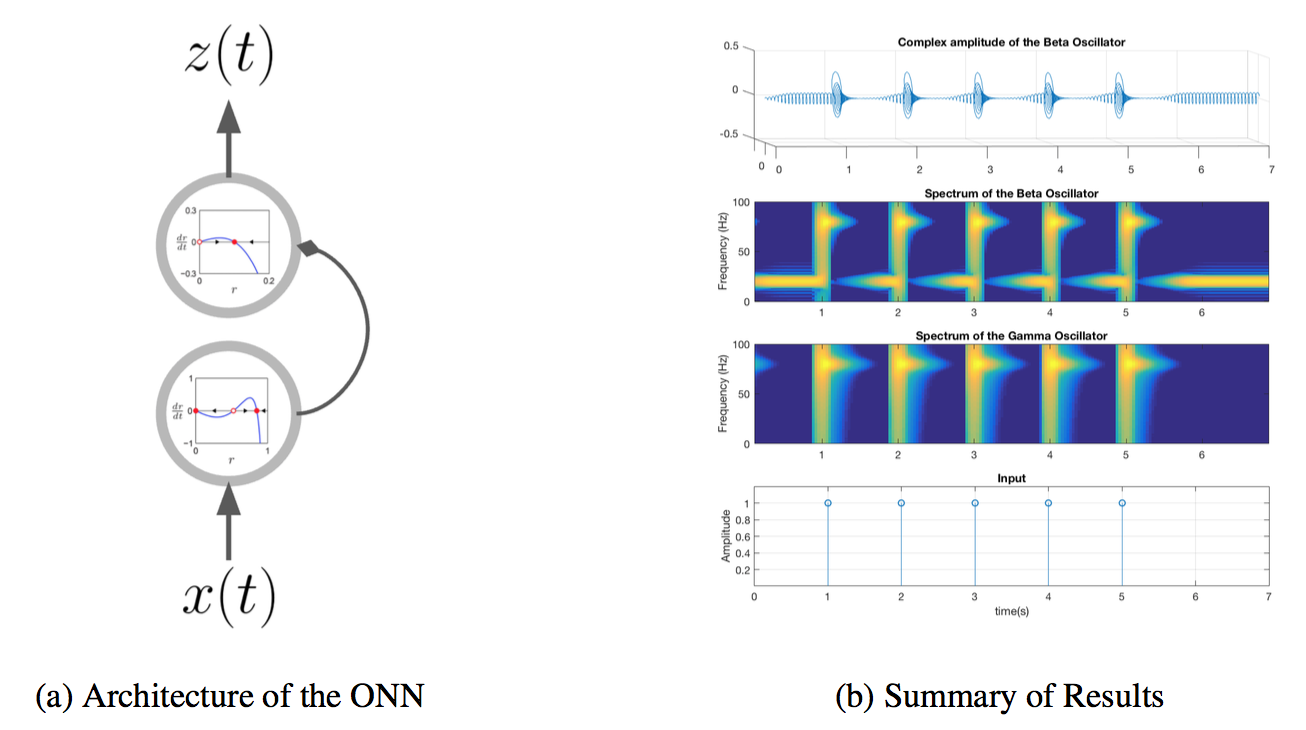
\includegraphics[scale=0.5]{arch1.png}
  \caption{Architecture (left) and summary of results (right)}
  \label{fig:arch1}
\end{figure}

Figure \ref{fig:arch1}a depicts our first architecture. The model contains a high-gamma oscillator (at 80Hz) that receives periodic impulses as input. The parameters of the high-gamma oscillator are $\alpha = -15$, $\beta_1 = 1$ $\beta_2 = -1$, and $epsilon = 1$, which make it a double-limit cycle oscillator capable of keeping a memory state after periodic stimulation. A beta oscillator receives inhibitory input from the gamma oscillator and has parameters $\alpha = 8$, $\beta_1 = -2000$, $\beta_2 = 0$, and $\epsilon = 0$, which pose it at a limit cycle that spontaneously oscillates. 

Figure \ref{fig:arch1}b shows the behavior of our model through a brief period of isochronous impulses. The top two rows show the complex amplitude response and the spectrogram, respectively, of the beta oscillator. The oscillator changes in amplitude upon receiving inhibitory input from the high- gamma oscillator, whose spectrogram is shown in the third row of the figure. The impulses, input to the high-gamma oscillator, are shown in the bottom row of the figure. These results are consistent with evidence from electrophysiology literature indicating that isochronous stimulation trigger a high-frequency burst, and a subsequent ERD of beta-band oscillation. Our model is also able to memorize the period of isochronous impulses after an extended interval of stimulation. One major shortcoming for this architecture is its inability to generalize this behavior to different periods of stimulation. This could be solved by using a gradient of oscillators at different frequencies in the first layer, instead of just a single oscillator.

\subsection{Architecture 2}

\begin{figure}[b]
  \centering
  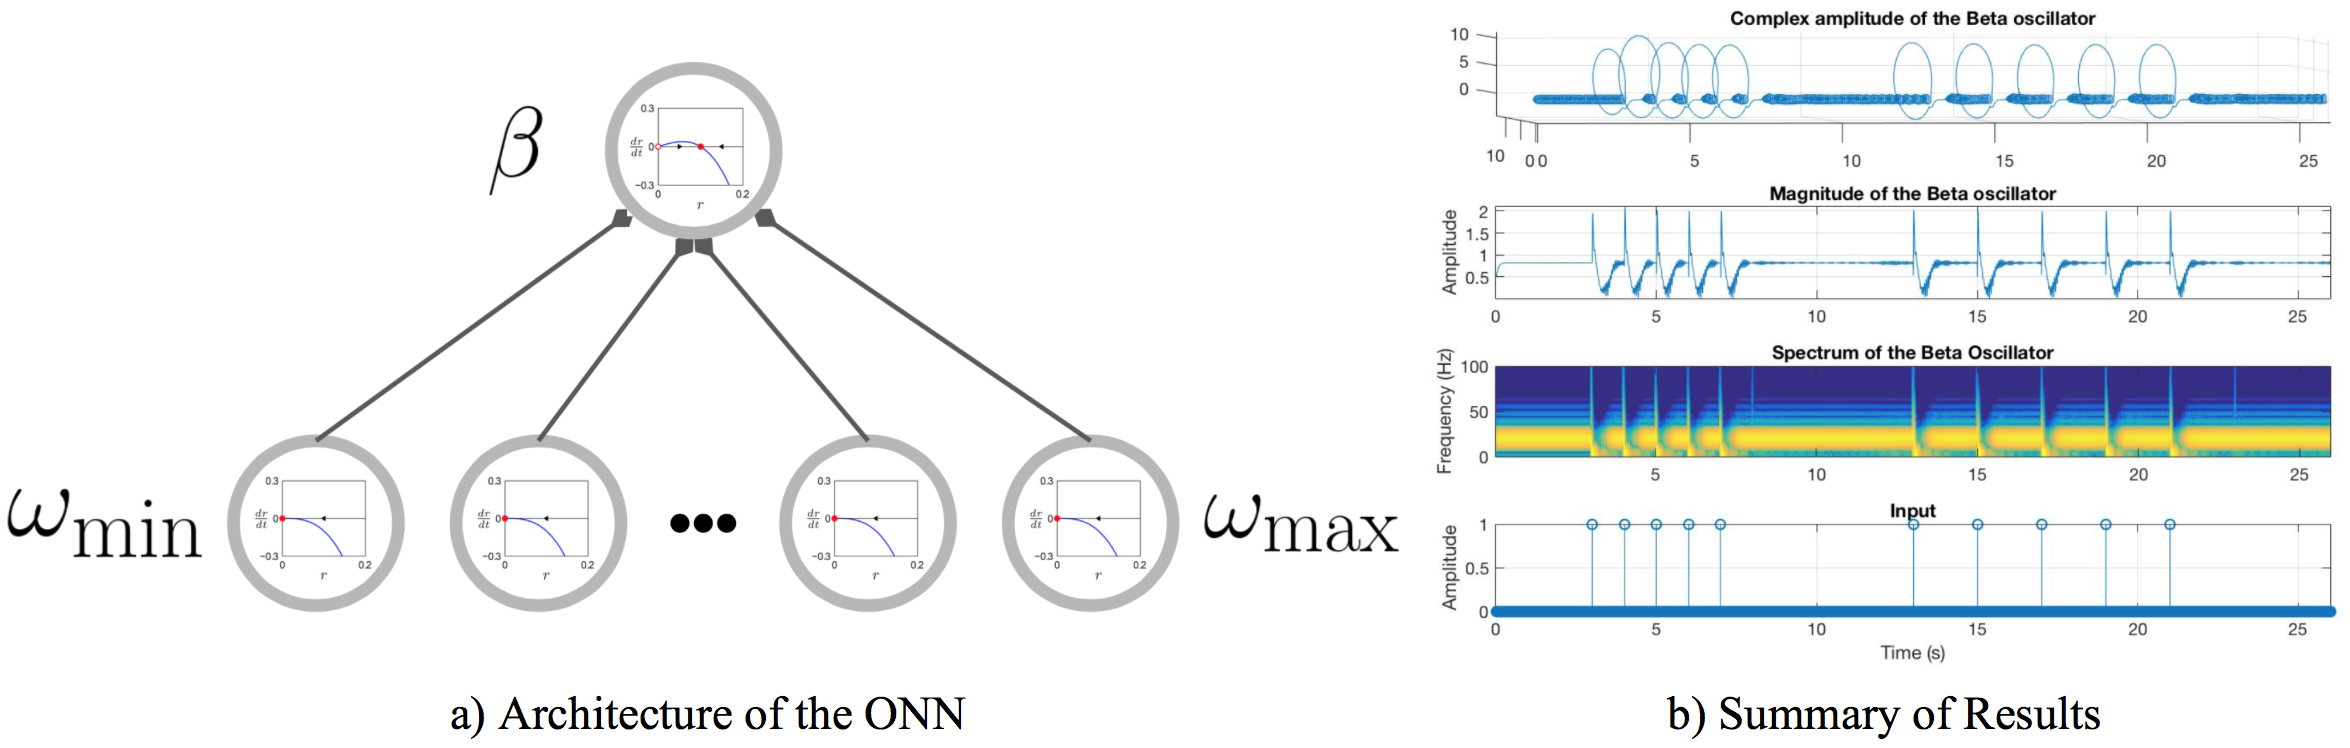
\includegraphics[scale=0.33]{arch2.png}
  \caption{Architecture (left) and summary of results (right)}
  \label{fig:arch2}
\end{figure}

Figure \ref{fig:arch2}a depicts our second architecture. Similar to previous models developed by Ed Large's group, our model's first later contains $N$ oscillators tuned to a gradient of logarithmically spaced frequencies going from $\omega_{min}$ to $\omega_{max}$. These oscillators are critical Hopf oscillators, which allows them to amplify inputs that make them resonate. This will make the second architecture able to process inputs with different periods of stimulation. The activity of the oscillators in the first layer is summed and passed as inhibitory input to the second layer, which contains a single oscillator tuned at 20Hz (beta band of brain oscillations).

Figure \ref{fig:arch2}b shows the behavior of our model through two periods of isochronous stimulation at two different frequencies. The top three rows show (in top-down order) the complex amplitude response, the magnitude, and the spectrogram of the beta oscillator. The oscillator changes in amplitude upon receiving inhibitory input from the first layer. The impulses, shown in the bottom row, are input to all the oscillators in the first layer. These results show that,  thanks to the gradient of frequencies, our model is able to process stimuli at different frequencies of stimulation, leading to the ERD in the beta layer. However, the rising slope through which the beta oscillator recovers its amplitude after the ERD does not anticipate the next stimulus, and remains constant regardless of the period of stimulation.

\subsection{Architecture 3}

Figure \ref{fig:arch3}a depicts our third architecture. In spirit, this architecture is very similar to architecture No2. Three major differences are: 1) The oscillators in the first layer are connected to (i.e. receive input from and send input to) the two oscillators neighboring them. 2) the output from all oscillators in layer one does not get added and passed as input to a single oscillator in the second layer. Instead, the second layer now contains the same number of oscillators as the first layer, and each oscillator in the first layer is connected to a single oscillator in the second layer. 3) The second layer now contains a gradient of slopes that will recover at different rates after an ERD. 

Figure \ref{fig:arch3}b shows the behavior of our model through two periods of isochronous stimulation at two different frequencies. The bottom row show the response of all the oscillators in the first layer to the periodic impulse. Notice how certain oscillators have larger amplitudes than others in response to the stimulation. This is due to the finer tuning resulting from oscillators in the first layer being connected to their neighbors. The middle row shows the behavior of an oscillator with a fast-recovering slope in the second layer, which properly anticipated the next beat during the faster period of stimulation, but not during the slower period of stimulation. The top row shows an oscillator with a slower slope of recovery, which properly anticipates the next stimulus during the slower stimulus (1st period of stimulation). During the second period of stimulation (faster), this same oscillator fails to anticipate the next beat.
\begin{figure}
  \centering
  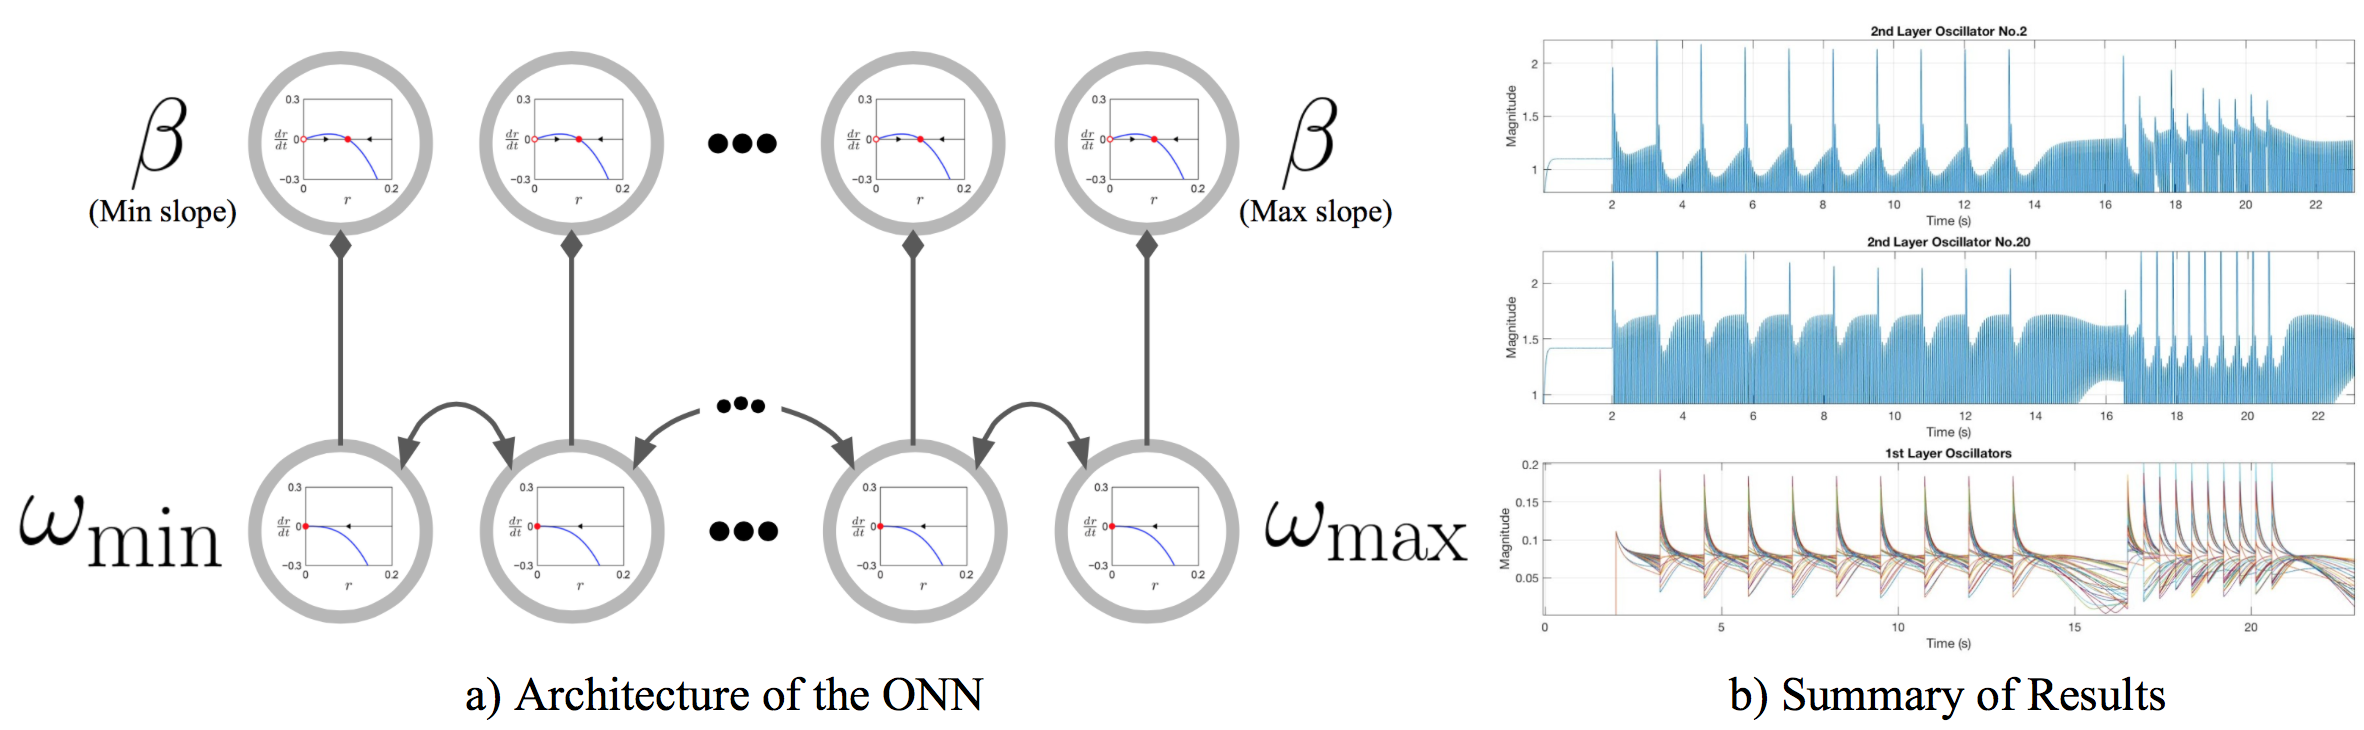
\includegraphics[scale=0.33]{arch3.png}
  \caption{Architecture (left) and summary of results (right)}
  \label{fig:arch3}
\end{figure}

\section{Conclusion and future work}

Canonical neural oscillators are able to capture the dynamics of ERDs as observed in the brain during periodic stimulation. The gradient of frequencies allowed the same architecture to process stimuli at different rates without having to change parameters. Thus, the signal processing capabilities of the model generalize across different rates of stimulation. The gradient of slopes also helped the model be able to capture the anticipatory quality of the ERD in the beta band. 

Considering the third model, the most sophisticated architecture presented here, the gradient of frequenices (1st layer) is biologically plausible due to the tonotopical organization of primary sensory areas in the cortex. However, it remains unclear whether the gradient of slopes in the second layer has a biological representation. More research about the mechanisms underlying brain oscillations in the motor cortex is needed to explain the cognitive mechanisms that relate anticipation and the ERDs observed in the motor cortex during periodic stimulation.

Finally, although the model generalizes to stimulation at different frequencies, the parameter space allowing for this behavior was found through fixed-point analysis and principles of oscillator design. Thus, the parameter search is not automated or data-driven. The realm of parameters involved in this canonical model is too complex, and a lack of control across bifurcation states could lead to the parameter search to get stuck at local-minima. However, with proper caution a cost-function-driven parameter search should be an immediate next step. The results outlined in this paper confirm that such parameter search could be carried out, although caution should be taken to avoid training of the model that remains stuck at qualitatively different dynamical states of the Hopf bifurcation.\\

The code is available \href{https://github.com/wisamreid/GrFNNMotor.git}{here}.

\bibliographystyle{apalike}
\bibliography{ref}

\end{document}
